\begin{comment}
\documentclass[10pt]{article}
\usepackage{fullpage, graphicx, url}
\setlength{\parskip}{1ex}
\setlength{\parindent}{0ex}
\title{GEN09}
\begin{document}


\begin{tabular}{ccc}
The Alternative Csound Reference Manual & & \\
Previous & &Next

\end{tabular}

%\hline 
\end{comment}
\section{GEN09}
GEN09�--� Generate composite waveforms made up of weighted sums of simple sinusoids. \subsection*{Description}


  These subroutines generate composite waveforms made up of weighted sums of simple sinusoids. The specification of each contributing partial requires 3 p-fields using \emph{GEN09}
. 
\subsection*{Syntax}


 \textbf{f}
 \# time size 9 pna stra phsa pnb strb phsb ...
\subsection*{Initialization}


 \emph{size}
 -- number of points in the table. Must be a power of 2 or power-of-2 plus 1 (see \emph{f statement}
). 


 \emph{pna, pnb}
, etc. -- partial no. (relative to a fundamental that would occupy \emph{size}
 locations per cycle) of sinusoid a, sinusoid b, etc. Must be positive, but need not be a whole number, i.e., non-harmonic partials are permitted. Partials may be in any order. 


 \emph{stra, strb}
, etc. -- strength of partials \emph{pna, pnb}
, etc. These are relative strengths, since the composite waveform may be rescaled later. Negative values are permitted and imply a 180 degree phase shift. 


 \emph{phsa, phsb}
, etc. -- initial phase of partials \emph{pna, pnb,}
 etc., expressed in degrees (0-360). 


 


\begin{tabular}{cc}
\textbf{Note}
 \\
� &

 


 
\begin{itemize}
\item 

  These subroutines generate stored functions as sums of sinusoids of different frequencies. The two major restrictions on \emph{GEN10}
 that the partials be harmonic and in phase do not apply to \emph{GEN09}
 or \emph{GEN19}
. 


  In each case the composite wave, once drawn, is then rescaled to unity if p4 was positive. A negative p4 will cause rescaling to be skipped. 


\end{itemize}


\end{tabular}

\subsection*{Examples}


  Here is a simple example of the GEN09 routine. It uses the files \emph{gen09.orc}
 and \emph{gen09.sco}
. It will generate a cosine wave, a sine wave with an initial phase of 90 degrees. Here is its diagram: 


 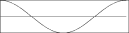
\includegraphics[scale=1]{gen09} 


 Diagram of the waveform generated by GEN09.


 \textbf{Example 1. A simple example of the GEN09 routine.}

\begin{lstlisting}
/* gen09.orc */
; Initialize the global variables.
sr = 44100
kr = 4410
ksmps = 10
nchnls = 1

; Instrument #1.
instr 1
  kamp = 30000
  kcps = 440
  ifn = 1

  ; Play the waveform stored in Table #1.
  a1 oscil kamp, kcps, ifn
  out a1
endin
/* gen09.orc */
        
\end{lstlisting}
\begin{lstlisting}
/* gen09.sco */
; Table #1: a cosine wave (using GEN09).
; This is a sine wave with an initial phase of 90 degrees.
f 1 0 16384 9 1 1 90

; Play Instrument #1 for 2 seconds.
i 1 0 2
e
/* gen09.sco */
        
\end{lstlisting}


  Here is another example of the GEN09 routine. It uses the files \emph{gen09square.orc}
 and \emph{gen09square.sco}
. It combines partials l, 3 and 9 in the relative strengths in which they are found in a square wave, except that partial 9 is upside down. It will be rescaled, here is its diagram: 


 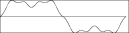
\includegraphics[scale=1]{gen09square} 


 Diagram of the waveform generated by GEN09.


 \textbf{Example 2. A square wave generated by the GEN09 routine.}

\begin{lstlisting}
/* gen09square.orc */
; Initialize the global variables.
sr = 44100
kr = 4410
ksmps = 10
nchnls = 1

; Instrument #1.
instr 1
  kamp = 30000
  kcps = 440
  ifn = 1

  ; Play the waveform stored in Table #1.
  a1 oscil kamp, kcps, ifn
  out a1
endin
/* gen09square.orc */
        
\end{lstlisting}
\begin{lstlisting}
/* gen09square.sco */
; Table #1: an approximation of a square wave (using GEN09).
f 1 0 16384 9 1 3 0 3 1 0 9 0.3333 180

; Play Instrument #1 for 2 seconds.
i 1 0 2
e
/* gen09square.sco */
        
\end{lstlisting}
\subsection*{See Also}


 \emph{GEN10}
, \emph{GEN19}

\subsection*{Credits}


 The simple example was written by Kevin Conder.
%\hline 


\begin{comment}
\begin{tabular}{lcr}
Previous &Home &Next \\
GEN08 &Up &GEN10

\end{tabular}


\end{document}
\end{comment}
